Dada una preforma, calcular cuantos metros del núcleo de un cable de fibra óptica se puede producir con las siguientes características:
\begin{figure}[H]
\centering
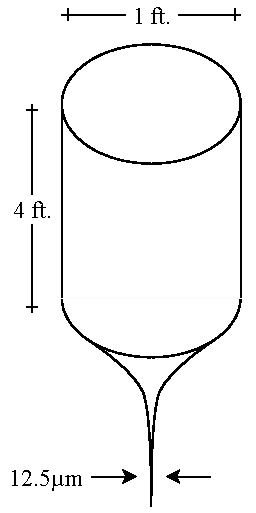
\includegraphics[page=1,scale=0.8]{PreformaImg.pdf}
\end{figure}
Calculamos algunos datos previos, viendo la preforma y una seccion de un metro de fibra como cilindros: \\{ }\\
\begin{minipage}[t]{.5\textwidth}
\raggedright
\subsubsection*{Preforma}
$r_p=0.5 ft. = 0.1524m$ \\
$h_p=4.0 ft. = 1.2192m$
\end{minipage}% <---------------- Note the use of "%"
\begin{minipage}[t]{.5\textwidth}
\raggedright
\subsubsection*{Fibra}
$r_f=62.5\mu m=62.5\times 10^{-6}m$ \\
$h_f=1m$
\end{minipage}% <---------------- Note the use of "%"
\\{ }\\
Para ambas calculamos el columen del cilindro que representa:
\\{ }\\
\begin{minipage}[t]{.5\textwidth}
\raggedright
\subsubsection*{Volumen Preforma}
$$
V_p = \pi \cdot r_p^2 \cdot h_p
$$
\end{minipage}% <---------------- Note the use of "%"
\begin{minipage}[t]{.5\textwidth}
\raggedright
\subsubsection*{Volumen Seccion de Nucleo (1m)}
$$
V_f = \pi \cdot r_f^2 \cdot h_f
$$
\end{minipage}% <---------------- Note the use of "%"
\\{ }\\
Por lo tanto la cantidad de metros($n$) que se pueden producir con esta preforma es:

$$
	n = \dfrac{V_p}{V_f} = \dfrac{\pi \cdot r_p^2 \cdot h_p}{\pi \cdot r_f^2 \cdot h_f} = \dfrac{r_p^2 \cdot h_p}{r_f^2 \cdot h_f} = \dfrac{0.1524^2 \cdot 1.2192}{(62.5\times 10^{-6})^2 \cdot 1} m = 7249112.728 m (7249.1127Km)
$$